\subsection{Age of Mothers}
Our first aim was to have an overall understanding of the mothers' age group and their proportions. After performing some statistical analysis we get two figures that show the trends of mothers of different age groups in different states as well as overall Australia. It can be observed that in most Australian states women who are aged less than 20 make the most proportion of mothers. After them, mothers who are 40 or more make up the 2nd largest age group (figure \ref{fig:age0.1}). Mothers from the age group of 20-24 make up the second biggest sample if we look at individual data from different states (figure \ref{fig:age0.2}). However, in (Figure: \ref{fig:age1}) ACT we see a different trend in data. We can see that the age group of 15-19 and over 40 are the last 2 age groups while most mothers are from the age group of 30-34. 

\begin{figure}
  \centering
  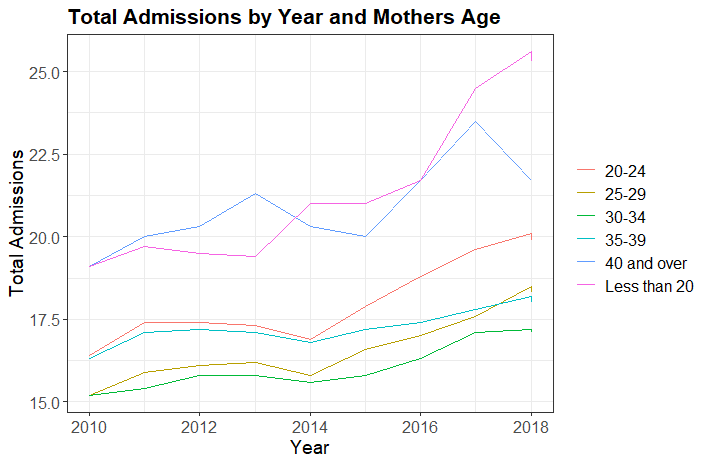
\includegraphics[width=1\textwidth]{subsections/age_mothers/mothers_age.png}
  \caption{Proportion of mothers by different age groups in Australia.}
  \label{fig:age0.1}
\end{figure}

\begin{figure}
  \centering
  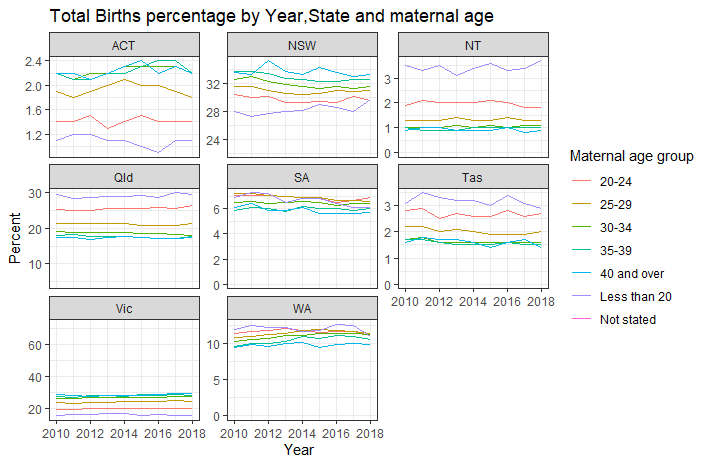
\includegraphics[width=1\textwidth]{subsections/age_mothers/birth_age_state.png}
  \caption{Proportion of mothers by different age groups in different states.}
  \label{fig:age0.2}
\end{figure}

\begin{figure}
  \centering
  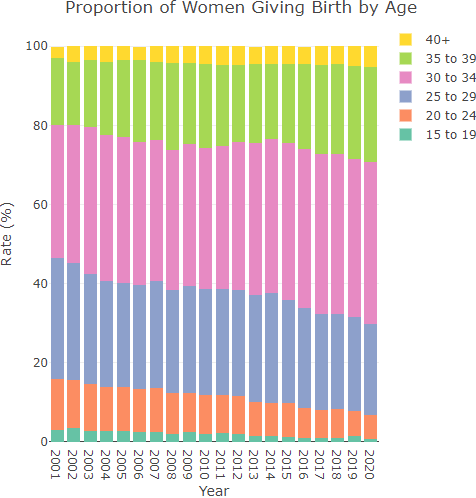
\includegraphics[width=0.50\textwidth]{subsections/age_mothers/age_group.png}
  \caption{Proportion of woman giving birth by age in ACT.}
  \label{fig:age1}
\end{figure}
\subsubsection{Analysis: First Time Mothers of ACT}

\begin{figure}
  \centering
  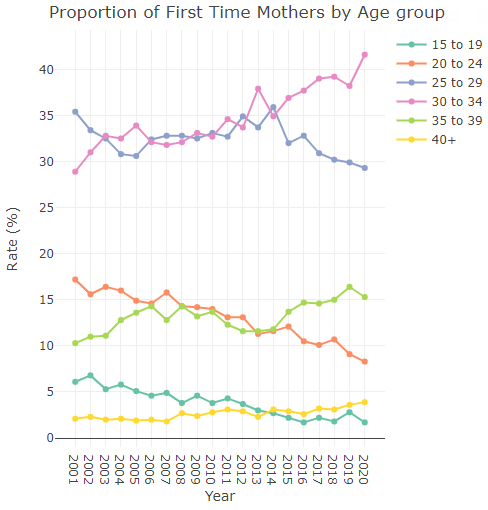
\includegraphics[width=0.5\textwidth]{subsections/age_mothers/first_time_age_group.png}
  \caption{Trends of first-time mother by age group.}
  \label{fig:age2}
\end{figure}

\begin{figure}
  \centering
  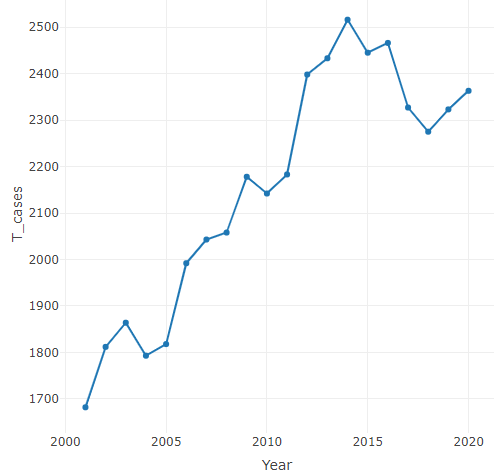
\includegraphics[width=0.45\textwidth]{subsections/age_mothers/first_time.png}
  \caption{Number of first-time mothers in each year.}
  \label{fig:firstTime}
\end{figure}
For a deeper understanding of what we have found in \verb|section 5.2| we were interested to see how many women became mothers for the first time. To achieve that we have generated Figure: \ref{fig:age2} where we can see that although mothers who are aged 40+ tend to have babies less the trend has been changing from the last decade and they have more birthrate than the age group of 15-19 years old. The low birthrate of 15-19 is understandably low as the legal age of consent is 16 except for Tasmania and South Australia which is 17 \cite{consentWebsite}.

Intuitively, this analysis leads us to ask how many women were becoming mothers for the first time each year so that we can observe a trend in women having babies. After generating figure: \ref{fig:firstTime} we can see that number of women becoming first-time mothers has increased over the years.
